%%%%%%%%%%%%%%%%%%%%%%%%%%%%%%%%%%%
%%  Einführung
%%%%%%%%%%%%%%%%%%%%%%%%%%%%%%%%%%%
\section*{Einführung ins Thema}

Die Wetterstation Arbon wurde 2004 als Lehrlingsarbeit des Berufsbildungszentrums Arbon auf Initiative der Technischen Gesellschaft Arbon (TGA) aufgebaut und in Betrieb genommen. Sie besteht aus mehreren Wettersensoren und einer Webcam, die auf einer Plattform auf dem See draussen montiert sind. Die Messwerte werden auf der Webseite\footnote{ \url{https://www.wetter-arbon.ch}}  der Wetterstation Arbon angezeigt.

\begin{figure}[h!]
	\centering
	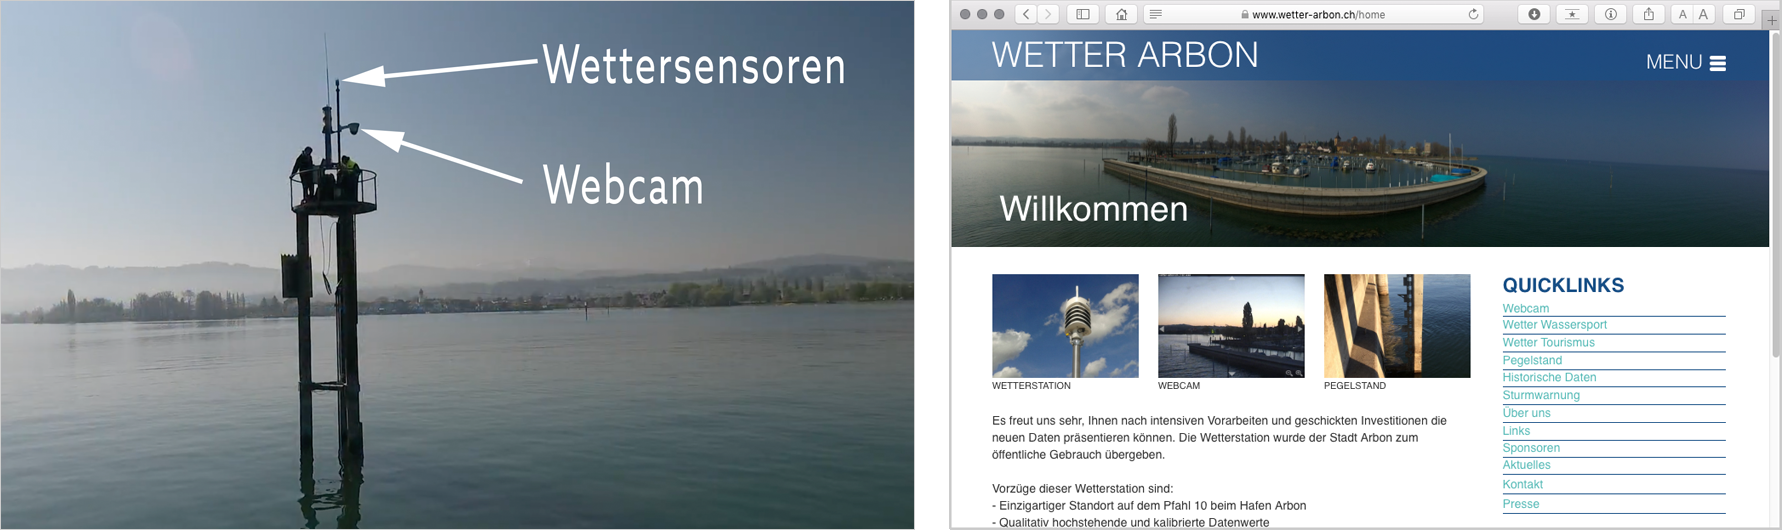
\includegraphics[width=1\linewidth]{img/kombi}
	\caption{Installation und Webseite der Wetterstation Arbon}
	\label{img:wetterstation}
\end{figure}

Was damals modern war, ist heute veraltet. Sowohl auf der Hardwareseite, als auch auf der Webseite gibt es diverses Reparatur- beziehungsweise Modernisierungspotential. Die Bachelor-Arbeit hat das Ziel, die Wetterstation wieder auf einen modernen, vollfunktionsfähigen Stand zu bringen. Während des Fachmoduls, welches die Vorbereitung für die Bachelor-Arbeit darstellt, führten wir eine Ist-Aufnahme der Wetterstation Arbon durch. Im Fokus lag sowohl die Hardware als auch die Software. Der Übersicht halber und damit wir die Arbeiten besser untereinander aufteilen konnten, haben wir die Themen in die vier Blöcke:  Webseite, Datenbank, Sensoren und Webcam unterteilt. (vgl. Abb. \ref{img:module})

\vspace{5mm} %5mm vertical space

\begin{figure}[h!]
	\centering
	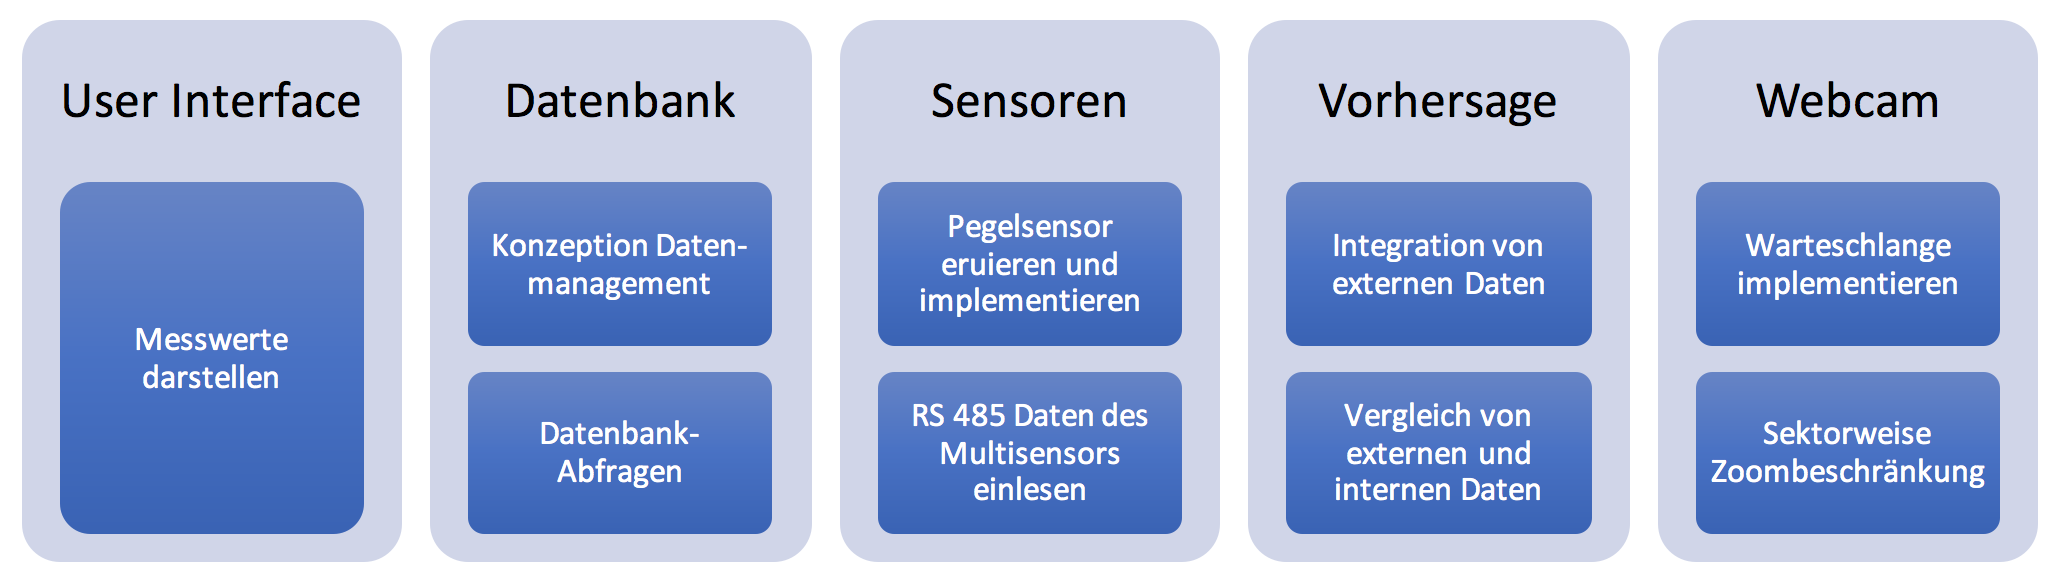
\includegraphics[width=0.8\linewidth]{img/module.pdf}
	\caption{Aufteilung in Arbeitsblöcke}
	\label{img:module}
\end{figure}

Pro Block wird jeweils aufgezeigt, wie die jetzige Situation ist, wo die Problemstellen liegen und wie die Lösungsansätze aussehen. Neben der Ist-Analyse haben wir uns Gedanken gemacht, wie der Funktionsumfang der Wetterstation erweitert werden kann. Die Ideen dazu sind im Abschnitt \flqq Erweiterungen\frqq aufgeführt. Die Erkenntnisse des Fachmoduls und insbesondere die Anforderungen dienen als Grundlage für die Bachelor-Arbeit. Dort geht es darum, die Lösungsansätze zu konkretisieren und gemäss den Anforderungen umzusetzen.

\newpage
